\documentclass[../main/main.tex]{subfiles}
\begin{document}
\mainmatter

\dominitoc
\faketableofcontents
\dominilof
\fakelistoffigures
\dominilot
\fakelistoftables

\chapter{Contexte cosmologique}\label{ch:cosmo}

\epigraph{\openquote\textit{Time is an illusion, a construct made out of human
memory}\closequote}{Blake \textsc{Crouch}, \textit{Revelations}}

Bien que la cosmologie ne s'en tienne pas aux concepts récents tels que nous les
connaissons et les vulgarisons, c'est avec les travaux d'\textsc{Einstein} au
début du XX\ieme~siècle que notre compréhension du monde cosmique se développe
de manière vertigineuse. Ces découvertes ont radicalement changé notre
appréhension de la structure et de l'histoire de notre Univers, dans la
continuité de la révolution copernicienne nous retirant du centre du monde~:
avec les fondements de la Relativité Générale, il n'y a non seulement aucun
point privilégié dans l'Univers, mais le temps même devient relatif à
l'observation.

Dans ce chapitre, nous donnons quelques notions et éléments de contexte
permettant de comprendre comment les SNe~Ia s'intègrent à la cosmologie
observationnelle moderne. Ainsi, dans la première section (\ref{sec:bases}) nous
discutons des bases nécessaires de relativité générale, qui nous mènera dans la
deuxième section (\ref{sec:MS}) au modèle cosmologique le plus robuste et qui
constitue la base de notre description du monde aujourd'hui. Enfin, nous verrons
dans la troisième et dernière section de ce chapitre (\ref{sec:dist}) quelles
sont les grandeurs d'intérêt à la cosmologie observationnelle et comment les
SNe~Ia permettent d'agrandir notre connaissance sur l'Univers.

\vfill
\minitoc
\vfill

\newpage

\section{Bases de relativité générale}\label{sec:bases}

Nous introduisons dans cette section les idées et grandeurs fondamentales à la
description de l'Univers par la relativité générale. Elle n'a pas pour vocation
de détailler intégralement les idées de mécaniques classiques sur lesquelles
elles se basent, mais de donner une idée des changements qu'elle implique.

\subsection{Concepts initiaux}\label{ssec:RG}

La relativité générale augmente les idées déjà introduites par la relativité
restreinte \citep[voir][et les autres articles de l'\textit{annus
mirabilis}\footnote{c'est ainsi que nous nommons l'année 1905 pendant laquelle
    \textsc{Einstein} publie quatre articles considérés comme étant à l'origine
de la physique moderne}]{einstein1905}, à savoir~:
\begin{enumerate}
    \item Les lois de la physique (\textit{hormis la gravitation}) sont
        invariantes par changement de référentiel galiléen\footnote{en quelques
            mots, nous pouvons traduire un référentiel comme um observataire,
            c'est-à-dire un lieu de mesure de distances et de durées de
            référence~; il est dit «~galiléen~», ou «~inertiel~», quand il n'est
            pas en accélération~: il peut l'être à une vitesse constante par
            rapport à un autre référentiel, c'est le cas d'un train à vitesse
        fixe et du paysage qu'il traverse}~;
    \item La vitesse de la lumière dans le vide est identique dans tous les
        référentiels galiléens.
\end{enumerate}

Ces hypothèses, qui n'ont peut-être \textit{a priori} pas l'air
révolutionnaires, sont le fondement de notre conception du monde physique
actuel. D'une part, aucun point et aucune direction de l'espace n'est
particulière dans le cadre du fonctionnement des lois de la
physique\footnote{nous disons dit que les lois de la physique sont
\textit{homogènes} et \textit{isotrope}, respectivement} (l'Univers entier même
n'a donc pas de centre~!), et d'autre part pour chaque observataire la mesure de
la vitesse de la lumière sera la même, peu importe sa propre vitesse. C'est
subtilement affirmer que cette vitesse est infranchissable, définissant des
espaces qui sont non causalement reliés entre eux (ils ne peuvent interagir l'un
avec l'autre) et que les lois physiques sont décrites en quatre dimensions
(trois d'espace et une de temps), mais aussi que la lumière est la référence
absolue de communication.

Ensemble, ces deux postulats permettent de mettre en évidence que pour relier
deux événements dans des référentiels inertiels différents, une simple
translation\footnote{c'est-à-dire l'ajout d'une distance à une autre} ne suffit
plus. En effet, en mécanique classique si une personne sur un train très rapide
allume une lampe vers l'arrière du train, une personne sur le quai dudit train
estimerait à la baisse la vitesse de cette lumière (elle serait même nulle si le
train allait à la vitesse de la lumière), par additivité des vitesses. Ceci
n'est pas possible en relativité restreinte, et les transformations amenant d'un
référentiel à l'autre ne sont pas linéaires avec la vitesse\footnote{nous les
appelons les \textit{transformations de \textsc{Lorentz}}, du nom du
mathématicien à l'origine de leur définition~: ça n'est en effet pas
\textsc{Einstein} le premier a avoir, par exemple, postulé que $E = mc^2$~:
c'est le premier à avoir regroupé les principes de la relativité en un
concept simple}. La relativité restreinte nous indiquerait qu'en réalité, du
point de vue du quai le temps dans le wagon du train s'écoule plus
lentement\footnote{la démonstration est laissée à læ lectaire investix…}, une
aberration en mécanique classique. Si ceci n'avait jamais été postulé, c'est que
les effets sont minimes aux vitesses que nous connaissons, et les variations
bien plus faibles que ce que nos instruments pouvaient mesurer alors\footnote{il
faudrait aller à 85\% de la vitesse de la lumière, soit $\approx
\SI{260000}{km.s^{-1}}$, pour dilater le temps d'un facteur 2}. Parmi les
conséquences peu intuitives en plus de la dilatation des durées, nous pouvons citer
la relativité de la simultanéité\footnote{deux événements à deux endroits
différents qui sont simultanés dans un référentiel ne le sont en général pas
dans un autre référentiel en mouvement par rapport au premier} et la contraction
des longueurs.

Avec la relativité générale, le premier principe cité s'élargit et un nouveau
principe, dit d'«~équivalence~», est introduit~:
\begin{enumerate}
    \item les lois de la physique (gravité comprise) sont identiques dans
        \textit{tous} les référentiels~;
    \item la force gravitationnelle sur un corps est équivalente à une
        accélération du référentiel associé audit corps.
\end{enumerate}
Celui-ci est aussi parfois exprimé sous la forme «~les masses graves et inertes
sont égales~»~: nous pouvons en effet définir la masse comme le facteur à
l'origine de l'attraction gravitationnelle (masse grave) mais aussi comme le
facteur traduisant l'inertie d'un système (masse inertielle), c'est-à-dire sa
facilité à changer de vitesse. Un référentiel en chute libre dans un champ de
gravitation est alors un référentiel inertiel (où la relativité restreinte
s'applique).

Ici aussi, si ces idées n'ont pas l'air révolutionnaires, leurs implications
sont nombreuses. Notamment, pour correspondre à la relativité restreinte qui
reste valable dans ce cadre, la mesure des longueurs dans un référentiel
accéléré (non galiléen) ne peut se définir dans un espace plat~: comme une bille
suit la courbe d'une cuvette en y tombant par l'effet de la gravité, la force
d'attraction gravitationnelle est le résultat d'une déformation même de
l'espace-temps forçant des objets massifs à se rapprocher. Ceci constitue une
autre révolution par rapport à la vision newtonienne de la force de gravité,
agissant avec une vitesse jusque-là considérée comme infinie et sans cause bien
définie. Dans ce cadre, les effets gravitationnels aussi mettent du temps à
parcourir l'espace, comme un tissu tendu déformé par une bille prend un certain
temps à reprendre sa forme quand celle-ci est enlevée.

Nous décrivons maintenant les grandeurs et équations décrivant la géométrie de
l'espace-temps en fonction de l'énergie qui y est appliquée.

\subsection{Métrique FLRW en Univers plat}\label{ssec:cons}

Les formalisme mathématique nécessaire pour décrire des espaces courbés en
quatre dimensions utilise des objets définis par la géométrie différentielles,
notamment les tenseurs. Ce sont des augmentations des matrices de rotation et
translation en 3D, qui associent à une grandeur sur une dimension une
combinaison des autres. Dans la pratique classique de la physique, nous
définissons une distance $\d L$ entre deux points $u=(x,y,z)$ et $v=(x',y',z')$
d'un espace orthonormé qui vérifie\footnote{c'est le théorème de
\textsc{Pythagore} en 3D}
\begin{equation}
    (\d L)^2 = (\d x)^2 + (\d y)^2 + (\d z)^2
\end{equation}
avec $\d p = p'-p$ pour $p = x,$ $y$ ou $z$, et nous pouvons définir de manière
indépendante un durée $\d t$ entre deux événements survenant à $t$ et $t'$ telle
que $\d t = t'-t$. Nous écrivons de manière compacte pour la première
\begin{equation}
    (\d L)^2 = \d w^T\left(\begin{array}{c c c}
            1 & 0 & 0\\
            0 & 1 & 0\\
            0 & 0 & 1\\
    \end{array}\right)\d w
\end{equation}
avec $\d w = v-u$ et $\d w^T$ sa transposée. Cette matrice diagonale ne mélange
pas les dimensions entre elles, et est souvent omise puisqu'elle décrit un effet
nul sur les coordonnées de l'espace, sans rotation ou translation~: une
modification de cette matrice traduirait une modification de la géométrie entre
ces deux points.

Dans un espace-temps plat à quatre dimensions, la «~distance~» entre deux
événements caractérisés par $u=(t,x,y,z)$ et $v=(t',x',y',z')$ est notée $\d s$
et vérifie
\begin{equation}
    (\d s)^2 = -(c\,\d t)^2 + (\d x)^2 + (\d y)^2 + (\d z)^2
\end{equation}
avec $c$ la vitesse de la lumière dans le vide. Cette construction a comme
particularité d'être nulle pour deux points sur le trajet d'un rayon
lumineux\footnote{en effet, le temps est dilaté à l'infini pour un corps
voyageant à la vitesse de la lumière}.

En notant $x^\mu$ les coordonnées d'un événement quadri-dimensionnel avec $\mu$
allant de 0 à 3, tel que $x^0 = ct$, $x^1 = x$ etc., cette égalité peut
également s'écrire de manière compacte, sous la forme
\begin{equation}
    (\d s)^2 = g_{\mu\nu}\d x^\mu \d x^\nu
\end{equation}
C'est cette grandeur $g_{\mu\nu}$ que nous appelons «~métrique~», et qui définit
la géométrie, courbe ou non, de notre espace. Dans le cas d'un espace plat, nous
voyons qu'elle se définit comme
\begin{equation}
    g_{\mu\nu} = \left(\begin{array}{c c c c}
            -1 & 0 & 0 & 0\\
            0 & 1 & 0 & 0\\
            0 & 0 & 1 & 0\\
            0 & 0 & 0 & 1\\
    \end{array}\right)
\end{equation}
et le chemin le plus court entre deux points est alors définit par une ligne
droite. Une métrique différente de celle-ci décrit un espace dans lequel le
chemin le plus court entre deux points est définit par une courbe dite
«~géodésique~». Assez intuitivement, même si c'est en quatre dimensions, plus la
métrique s'écarte de cette diagonale $(-1,+1,+1,+1)$ plus la géodésique sera
courbée.

Il faut cependant distinguer la courbure de l'Univers-même et la courbure
induite à l'espace-temps par la matière, par exemple. Dans notre cas, nous
supposons un Univers plat (ce qui semble être le cas d'après les mesures), mais
lui laissons la possibilité de varier en taille. S'il n'est pas possible de la
mesurer de manière absolue, il nous suffit de prendre une échelle de distance
entre deux objets aujourd'hui à $t = t_0$ et d'en regarder l'évolution avec le
temps cosmique~; c'est ainsi que nous définissons le facteur d'échelle $a(t)$
tel que $a(t=t_0) = 1$, et de cette manière la métrique de cet Univers devient
celle de \textsc{Friedmann}-\textsc{Lemaître}-\textsc{Robertson}-\textsc{Walker}
(FLRW) dans le cas spécifique d'un Univers plat, c'est-à-dire
\begin{equation}
    g_{\mu\nu} = \left(\begin{array}{c c c c}
            -1 & 0 & 0 & 0\\
            0 & a^2 & 0 & 0\\
            0 & 0 & a^2 & 0\\
            0 & 0 & 0 & a^2\\
    \end{array}\right)
\end{equation}

L'introduction de ce facteur d'échelle permet de définir le taux d'expansion de
l'Univers, que nous appelons paramètre de \textsc{Hubble} $H(t)$, tel que
\begin{equation}\label{eq:hz}
    H(t) = \frac{\dot{a}}{a}\quad\text{avec}\quad\dot{a} = \dv{a}{t}
\end{equation}
et nous appelons constante de \textsc{Hubble} sa valeur aujourd'hui~; nous
notons $H(t=t_0) = H_0$. Notons également qu'une contraction ou dilatation de
l'espace-temps implique inévitablement la variation de la longueur d'onde d'un
photon avec le facteur d'échelle~; nous l'appelons \textit{redshift} pour
«~décalage vers le rouge~», et nous le notons $z$ tel que
\begin{equation}\label{eq:z}
    \frac{a_0}{a(t)} = \frac{\lambda_0}{\lambda_e} = 1+z
\end{equation}
avec $\lambda_e$ la longueur d'onde au moment de l'émission et $\lambda_0$ celle
mesurée à la réception.

\subsection{Équations phares et paramètres cosmologiques}\label{ssec:rgeq}

Si $g_{\mu\nu}$ est une grandeur mathématique utile, la réelle courbure physique
de l'espace-temps est définie par le tenseur d'\textsc{Einstein}, $G_{\mu\nu}$.
C'est une grandeur physique, continue et dérivable deux fois avec une divergence
nulle\footnote{autrement dit, qui conserve le volume}, qui est nulle quand la
courbure est nulle (redonnant les équations de \textsc{Newton} aux limites
classiques) et qui dépend de $g_{\mu\nu}$. Dans le formalisme de la relativité
générale, la courbure de l'espace-temps en un point est reliée à l'énergie en ce
point~; notamment, la masse (que nous pouvons définir en énergie) courbe
l'espace pour créer l'effet de gravitation. Cette énergie est définie par un
autre tenseur $T_{\mu\nu}$, appelé «~énergie-impulsion~», également une grandeur
physique de divergence nulle. Ces grandeurs sont alors reliées par l'équation
d'\textsc{Einstein}~:
\begin{equation}\label{eq:ein}
    G_{\mu\nu} = \frac{8\pi\mathcal{G}}{c^4}T_{\mu\nu}
\end{equation}
avec $\mathcal{G}$ la constante gravitationnelle de \textsc{Newton}~; cette
équation est sans doute l'une des équations les plus emblématiques et
fondamentales de la physique moderne, d'une élégance presque inégalée.

Cependant, cette équation amènera \textsc{Einstein} à se rendre compte qu'un
Univers composé uniquement de matière et de rayonnement ne pouvait donner un
Univers statique~: le facteur d'échelle $a$ était destiné à varier, et donc
l'Univers a avoir potentiellement un début et une fin. Cette découverte était
inconcevable dans sa conception du monde, et pour contrer ce phénomène il
modifia son équation~\ref{eq:ein} en y ajoutant une constante cosmologique
$\Lambda$ qui peut s'introduire d'un côté ou de l'autre du signe égal, tel que
\begin{equation}\label{eq:einlamb}
    G_{\mu\nu} + \Lambda g_{\mu\nu} = \frac{8\pi\Gc}{c^4}T_{\mu\nu}
    \Longleftrightarrow
    G_{\mu\nu} = \frac{8\pi\Gc}{c^4}T_{\mu\nu} - \Lambda g_{\mu\nu} 
\end{equation}

Si d'une manière purement mathématique les deux équations sont équivalentes,
leurs motivations physiques sont différentes~: dans le premier cas, cela revient
à modifier intrinsèquement les lois de la gravitation en y introduisant un
phénomène complètement décorrélé de l'aspect géométrique de sa manifestation~;
dans le second, ce terme serait une nouvelle source de champ gravitationnel, une
forme d'énergie ne se diluant pas et donc indépendante du temps. Le fait que ce
terme puisse être des deux côtés du signe «~=~» signifie que nous ne pouvons pas
distinguer son origine. S'il est revenu sur sa décision plus tard, son inclusion
reste toute fois intéressante et nous conservons ce terme quitte à le trouver
nul par la suite.

Pour décrire la composition de l'Univers en énergie \textit{via} $T_{\mu\nu}$,
nous utilisons le modèle du fluide parfait. Il est défini par deux quantités~:
$\rho$, sa masse volumique (ou d'une manière plus générale, sa densité
d'énergie)~; et $p$, sa pression hydrostatique (c'est-à-dire une force par unité
de surface sur des parois, imaginaires ici). L'isotropie de notre Univers
implique que ce tenseur est diagonal dans son référentiel de repos puisqu'il
n'y a pas de direction privilégiée à sa pression, et que les trois composantes
d'espace ont la même valeur $p/c^2$. Nous pouvons donc l'écrire
\begin{equation}
    T_{\mu\nu} = \left(\begin{array}{c c c c}
            \rho & 0 & 0 & 0\\
            0 & p/c^2 & 0 & 0\\
            0 & 0 & p/c^2 & 0\\
            0 & 0 & 0 & p/c^2\\
    \end{array}\right)
\end{equation}

Le fait que l'énergie soit conservée dans le temps se traduit par la divergence
nulle du tenseur énergie-impulsion, de telle sorte qu'un fluide parfait est
caractérisé par l'équation de conservation
\begin{equation}\label{eq:cons}
    \dot{\rho} = -3H\rho(1+w)
\end{equation}
avec $w \triangleq p/\rho c^2$ le paramètre d'état du fluide en question. En
effet, de cette équation différentielle nous déduisons
\begin{equation}\label{eq:rho}
    \rho(t) \propto a(t)^{-3(1+w)}
\end{equation}
et le fluide présentera des comportements variés selon la valeur de $w$~:
\begin{itemize}
    \item si $w=0$, c'est-à-dire $p=0$, nous aurons $\rho \triangleq \rho_M
        \propto a^-3$~: c'est le comportement typique de la matière
        non-relativiste qui se déplace à faible vitesse et a donc une pression
        négligeable tout en ayant une densité d'énergie non-nulle se diluant
        avec le volume~;

    \item si $w=1/3$, nous aurons $\rho \triangleq \rho_R \propto a^{-4}$~:
        c'est le comportement de la limite ultra-relativiste ($v \approx c$),
        propre à l'énergie de radiation comme celle des photons ou des
        neutrinos. Nous la décrivons comme un fluide dont la densité se dilue
        comme la matière non-relativiste (avec $\rho_M \propto a^{-3}$) mais
        dont la longueur d'onde s'étire également avec le facteur d'échelle,
        diminuant la densité d'énergie par un facteur $a^{-1}$ supplémentaire~;

    \item si $w=-1$, c'est-à-dire $p < 0$, nous aurions alors $\rho \propto a^0
        = \text{constante}$. Ce paramètre d'état décrirait alors un fluide à
        pression négative mais dont la densité d'énergie de se dilue pas avec le
        facteur d'échelle… autrement dit, un comportement qui pourrait convenir
        pour décrire l'effet énergétique de la constante cosmologique~; on
        qualifie une telle forme d'énergie de «~sombre~».
\end{itemize}

À partir de cette idée de fluide parfait et avec l'équation~\ref{eq:ein} dans le
cadre de la métrique FLRW dans un Univers plat, nous pouvons dériver une autre
équation fondamentale de la relativité générale, à savoir
\begin{equation}\label{eq:fried}
    H^2 \triangleq \left( \frac{\dot{a}}{a} \right)^2 =
    \frac{8\pi\mathcal{G}\rho}{3c^2} + \frac{\Lambda c^2}{3}
\end{equation}
que nous appelons équation de \textsc{Friedmann} \citep{friedmann1922}.

Pour simplifier cette forme, nous pouvons prendre sa valeur à $t = t_0$ pour
définir une densité dite «~critique~»~:
\begin{equation}
    \rho_c = \frac{3c^2H_0{}^2}{8\pi\mathcal{G}}
\end{equation}
et ainsi, selon la nature des fluides composant l'Univers, nous séparons les
différents $\rho$ pour obtenir la forme
\begin{equation}
    H^2 \triangleq \left( \frac{\dot{a}}{a} \right)^2 =
    H_0{}^2 \left[ \frac{\rho_R(t_0)}{\rho_c}\frac{\rho_R}{\rho_R(t_0)} +
                   \frac{\rho_M(t_0)}{\rho_c}\frac{\rho_M}{\rho_M(t_0)} +
                   \frac{\Lambda c^2}{3 H_0{}^2}
               \right]
\end{equation}

Comme $\rho_R \propto a^{-4}$, $\DS\frac{\rho_R}{\rho_R(t_0)} = \frac{a_0}{a}^4$,
et de même $\DS\frac{\rho_M}{\rho_M(t_0)} = \frac{a_0}{a}^3$~; nous pouvons
donc réécrire
\begin{equation}
    H^2 \triangleq \left( \frac{\dot{a}}{a} \right)^2 =
        H_0{}^2 \left[ \Omega_R \left( \frac{a_0}{a} \right)^4 +
                       \Omega_M \left( \frac{a_0}{a} \right)^3 +
                       \Omega_\Lambda \right]
\end{equation}
et finalement obtenir, avec l'équation~\ref{eq:z}~:
\begin{equation}\label{eq:h2}
    H^2 \triangleq \left( \frac{\dot{a}}{a} \right)^2 =
        H_0{}^2 \left[ \Omega_R \left( 1+z \right)^4 +
                       \Omega_M \left( 1+z \right)^3 +
                       \Omega_\Lambda \right]
\end{equation}
en notant $\Omega_X \triangleq \DS \frac{\rho_X(t_0)}{\rho_c}$ pour $X = R$ ou
$M$, et $\Omega_\Lambda = \DS \frac{\Lambda c^2}{3 H_0{}^2}$. Ce sont ces
densités réduites, dont la somme est égale à 1 par construction (autrement dit,
$\sum_i \Omega_i = 1$) que nous appelons \textit{paramètres cosmologiques}~; ils
constituent avec $H_0$ la base de l'histoire et de l'évolution de l'Univers
étant donné qu'ils caractérisent la variation du taux d'expansion (au carré).

\subsection{Modèle standard de la cosmologie~: \lcdm}\label{sec:MS}

Si jusque-là notre approche était générale et historique (sauf pour l'Univers
plat), nous effectuons un saut dans le futur pour discuter de la cosmologie
moderne. L'origine éventuel et le futur de l'Univers sont en effet régis par les
valeurs de ces paramètres cosmologiques, et si \textsc{Einstein} n'eût pas la
chance de vivre jusqu'à la fin du XX\ieme~siècle nous avons des valeurs de ces
paramètres. Notamment, \cite{riess1998} et~\cite{perlmutter1999} ont mesuré,
grâce à des SNe~Ia, les valeurs des paramètres cosmologiques $\Omega_i$. Leurs
résultats indiquent que l'énergie totale de l'Univers serait à 70\% de l'énergie
sombre, autrement dit une forme d'énergie qui ne nous est pas tangible et dont
nous n'avons que pu caractériser les effets à l'échelle de l'Univers entier~; le
reste de cette énergie est alors principalement de la matière, qui composerait
30\% de l'énergie de l'Univers. La Figure~\ref{fig:snlambda} présente la
contrainte apportée par~\cite{riess1998} sur les paramètres $\Omega_\Lambda$ et
$\Omega_M$ ainsi que les contraintes actuelles que les SNe~Ia permettent (nous
détaillons le principe de ces mesures dans la section suivante).

\sidecaptionvpos{figure}{c}
\begin{SCfigure}[1][ht]
    \centering
    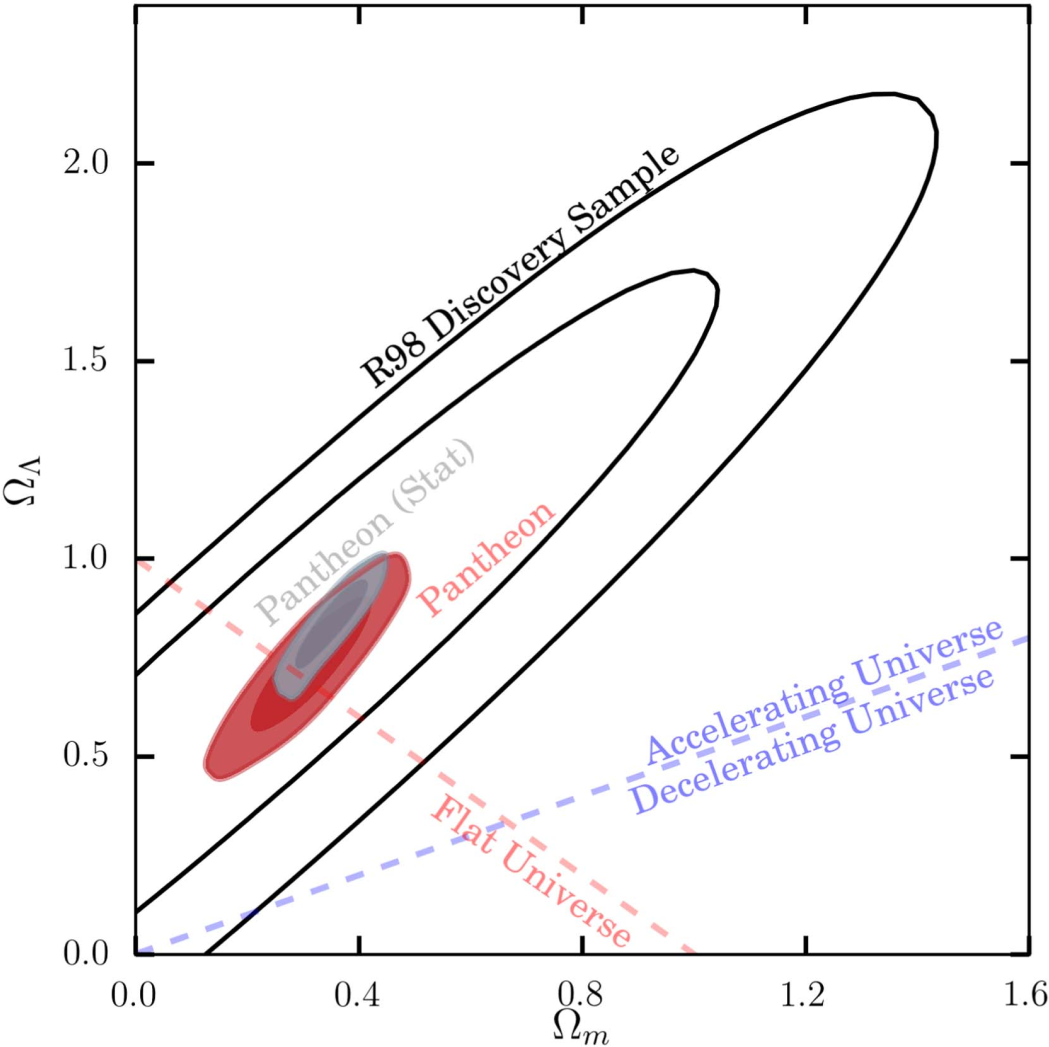
\includegraphics[width=.6\linewidth]{scolnic_snlambda}
    \caption[Contraintes sur les paramètres cosmologiques $\Omega_\Lambda$ et
    $\Omega_M$ par les SNe~Ia seulement]{Contraintes sur les paramètres
        cosmologiques $\Omega_\Lambda$ et $\Omega_M$ par les SNe~Ia seulement,
        mettant en évidence l'existence de l'énergie sombre. Les contours de
        confiance à 68 et 95\% sur les paramètres sont montrés pour les mesures
        de~\cite{riess1998} (R98 Discovery Sample) et celles de l'échantillon
        Pantheon \textit{en rouge}. Figure
    de~\cite{scolnic2018}.}\label{fig:snlambda}
\end{SCfigure}

Cette mesure implique la découverte de l'expansion accélérée de l'Univers, étant
donné qu'aucune autre forme d'énergie de rivalise actuellement avec celle-ci et
que, contrairement aux autres, sa densité ne se dilue pas avec le temps~;
autrement dit, l'Univers est voué, sauf preuve du contraire, à s'étendre
indéfiniment en isolant les structures qui ne sont pas en interaction
gravitationnelle suffisamment forte avec les autres. Cette découverte a mené
Saul \textsc{Perlmutter}, Adam \textsc{Riess} et Brian \textsc{Schmidt} a
obtenir le prix \textsc{Nobel} en 2011, après confirmation de ces mesures par
des sondes indépendantes permettant de mieux contraindre les paramètres
estimés\footnote{en effet, la mesure d'une distance avec une règle et avec le
    temps de vol d'un laser par exemple sont des méthodes de mesure qui
    permettent une estimation de la valeur attendue, mais reposent toutes les
    deux sur des principes physiques différents qui impliquent des dépendances
    et des erreurs qui se combinent pour mieux déterminer la longueur en
question}.

Le modèle vers lequel ces différentes sondes convergent est appelé le «~modèle
de concordance~». Sans les détailler, en dehors des SNe~Ia il existe des mesures
de ces paramètres cosmologiques \textit{via} le fonds diffus cosmologique
(\textit{Cosmic Microwave Background}, CMB) et les oscillations acoustiques des
baryons (\textit{Baryon Acoustic Oscillations}, BAO) notamment.
Ce modèle, dit «~standard~», décrit les observations de l'Univers \textit{via}
l'implication de matière sombre\footnote{c'est-à-dire une forme d'énergie
    similaire à la matière, avec un comportement gravitationnel attractif et un
    paramètre d'état $w=0$ mais invisible par rayonnement
électromagnétique} froide\footnote{on entend par là non-relativiste,
c'est-à-dire se déplaçant à des vitesses faibles devant celle de la lumière} et
d'une constante cosmologique $\Lambda$ (probablement sous forme d'énergie
sombre)~; il est pour cela appelé $\Lambda CDM$ pour \textit{Lambda Cold Dark
Matter}. Il permet de rendre compte de l'origine et de la structure du fonds
diffus cosmologique, de la composition en atomes et de la structure des grandes
échelles de l'Univers, ainsi que de son expansion accélérée. Si ses capacités
prédictives sont remarquables, la nature précise de la matière et de l'énergie
sombres reste pour le moment un mystère.

Il existe d'autres modèles de cosmologie, laissant certains paramètres varier~;
c'est le cas du modèle $w$CDM pour lequel le paramètre d'état de l'énergie
sombre n'est pas fixé à \num{-1}. Nous ne parvenons cependant pas encore à
réfuter l'un ou l'autre des modèles avec les mesures actuelles des paramètres~:
la combinaison SN+CMB+BAO de~\cite{scolnic2018} trouve en effet $w =
\num{-1.014}\pm\num{0.040}$, compatible avec $\Lambda$CDM. Nous présentons
Figure~\ref{fig:cosmocomb} les contraintes combinées de ces sondes pour $w$CDM.

\begin{SCfigure}[1][ht]
    \centering
    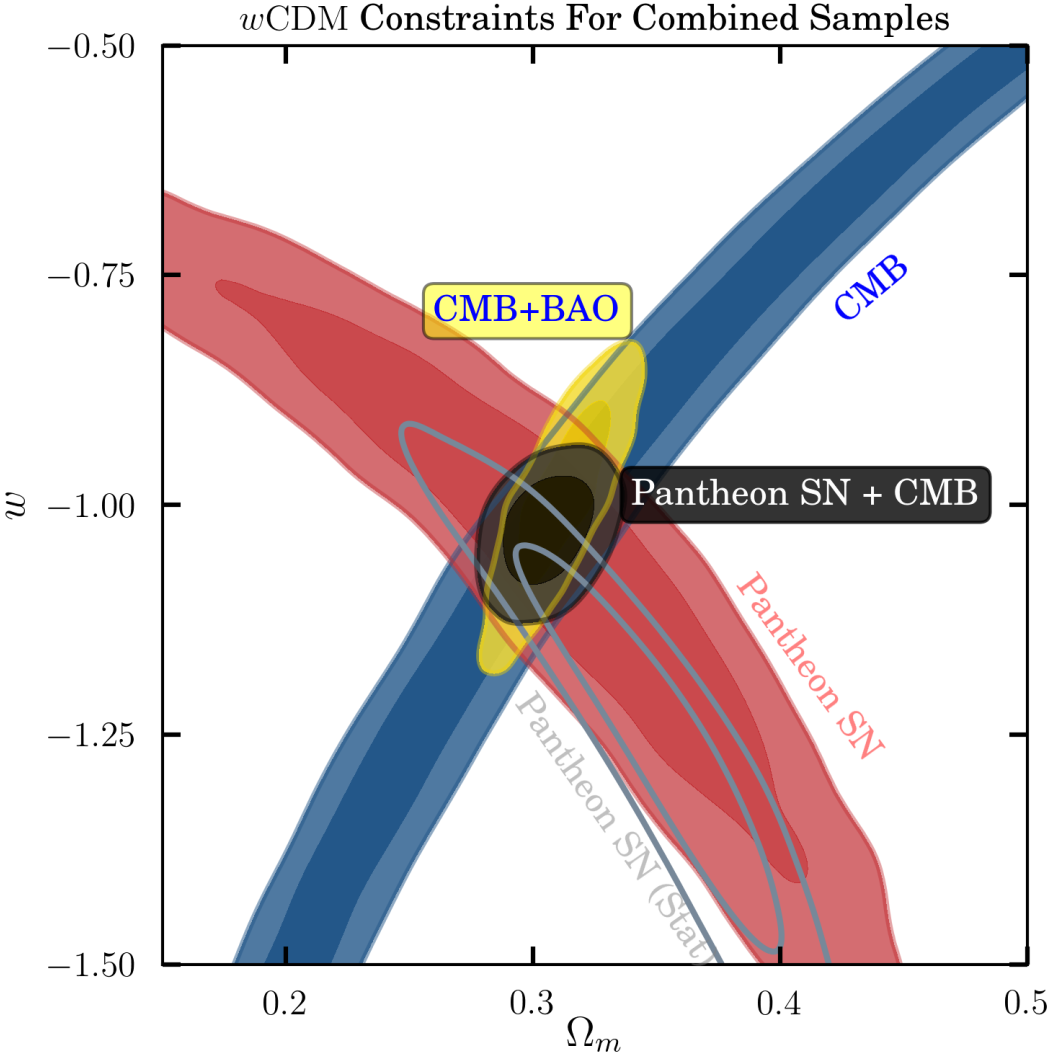
\includegraphics[width=.6\linewidth]{scolnic_combined}
    \caption[Contraintes sur les paramètres cosmologiques $w$ et $\Omega_M$ par
    la combinaison SNe~Ia, CMB et BAO]{Contraintes à 68 et 95\% sur les
        paramètres cosmologiques $w$ et $\Omega_M$ par la combinaison SNe~Ia
        (\textit{en rouge}), par le CMB (\textit{en bleu}) fournies par la
        collaboration~\cite{planck2015}. Les contours \textit{jaunes} combinent
        le CMB et le BAO~\citep{alam2015}~; les contours \textit{noirs} le CMB
    et les SNe~Ia. Figure de~\cite{scolnic2018}.}\label{fig:cosmocomb}
\end{SCfigure}
\sidecaptionvpos{figure}{t}

Il est cependant sujet à une tension historique du fait de l'incompatibilité de
la mesure de $H_0$ entre le CMB et les SNe~Ia~: en effet, ces deux méthodes
trouvent des valeurs respectives de \SI{67.4\pm0.5}{km.s^{-1}.Mpc^{-1}} et
\SI{73.04\pm1.04}{km.s^{-1}.Mpc^{-1}}. L'étude de cette incohérence est
actuellement au cœur de la cosmologie moderne, chacune de ces sondes ayant fait
ses preuves quant à leur fiabilité de mesures.

\section{Mesures cosmologiques}\label{sec:dist}

Nous discutons dans cette section des grandeurs qui servent un intérêt à notre
étude.

\subsection{Âge de l'Univers}\label{ssec:age}

Au cours du XX\ieme~siècle, l'expansion avérée de l'Univers a amené la
communauté scientifique à supposer qu'il devait exister, à une époque lointaine,
un état de l'Univers où son facteur d'échelle était infiniment proche de 0, soit
infiniment petit et donc infiniment chaud en concentrant toute l'énergie.
D'abord appelé de manière dérisoire \textit{Big Bang} en 1949 par un
astrophysicien qui contestait cette idée, cette idée a été confortée avec les
mesures qui ont suivi. Pour l'estimer, il nous faut faire correspondre le
facteur d'échelle avec le temps.

Nous utilisons pour cela le redshift $z$ d'un objet, qui est caractérisé par
l'équation~\ref{eq:z}, et la définition du taux d'expansion $H(z)$ de
l'équation~\ref{eq:hz}. Nous définissons alors l'âge de l'Univers comme celui
que l'on trouverait pour un corps de redshift infini. Nous pouvons le relier au
temps qu'il s'est écoulé entre son émission et sa réception par~:
\begin{align}
    t(z) & = \int_{0}^{t(z=\infty)} \d t' = \int_{0}^{a(z=\infty)} \frac{\d a'}{\dot{a}'}
    \nonumber\\
         & = \int_{0}^{a(z=\infty)} \frac{\d a'}{a'H(a')} = \int_{0}^{\infty} \frac{\d
         z'}{(1+z')H(z')}\nonumber\\
         & = \frac{1}{H_0} \int_{0}^{\infty} \frac{\d z'}{(1+z')E(z')}
\end{align}
où $E(z)$ se déduit de la définition de $H^2$ de l'équation~\ref{eq:h2}~:
\begin{equation}\label{eq:ez}
    E(z) \triangleq \frac{H(z)}{H_0} = \left[ \Omega_R(1+z)^4 + \Omega_M(1+z)^3
    + \Omega_\Lambda\right]^{1/2}
\end{equation}
L'âge de l'Univers dépend donc de la répartition de son énergie selon les
différentes formes qui le composent, c'est-à-dire du modèle~; dans le cadre du
modèle $\Lambda$CDM, il est estimé à $t_0 \SI{13.797\pm0.023}{Gans}$
par~\cite{planck2018}. Une modification de la fraction ou du paramètre d'état de
l'énergie sombre, notamment, amènerait à une variation de cette valeur.

\subsection{Distance de luminosité}\label{ssec:dl}

Si une variation de l'âge de l'Univers n'aurait pas grande incidence sur notre
rapport au monde, un effet notable de l'histoire de son expansion se remarque
sur les distances des sources lumineuses à nous. En effet,

\subsection{Intérêt des supernovae de type Ia}\label{ssec:intsne}

\newpage

\thispagestyle{plain}
% \vspace*{-3cm}
\vfill
\minilof
\vfill
\minilot
\vfill

\bibliographystyle{../main/aa_url}
\shorthandoff{:}
\bibliography{../chapters/99_references}

\end{document}
